
\section{Dataset }
%
\subsection{Curated USG Video Dataset for GBC Detection}
%
\begin{figure}[t]
    \centering
    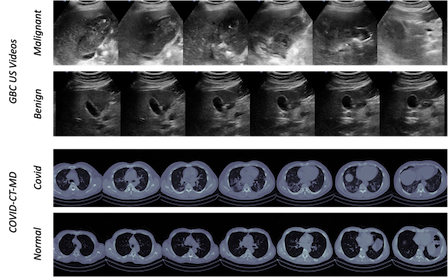
\includegraphics[width=0.85\linewidth]{figs/focusmae/data_sample_med.png}
    \caption[Sample video sequences from the USG and CT datasets]{Sample video sequences from our USG video dataset used for GBC detection, and the public COVID-CT-MD dataset \cite{covidctmd}. We show samples of both malignant and benign (non-malignant) sequences for GBC data. For the covid data, we show sample sequences for both Covid and non-Covid categories.}
    \label{focusmae_fig:data_sample}
\end{figure}
\mypara{Video Data Collection and Curation}
%
We utilized both the public Gallbladder USG video dataset (GBUSV) \cite{basu2022unsupervised} and an additional set of USG videos collected by our team of radiologists. The GBUSV dataset comprises 64 Gallbladder USG videos, with 32 labeled as benign and another 32 labeled as malignant. To augment our dataset for the video-based \gbc detection task, we incorporated 27 additional USG videos specifically depicting Gallbladder malignancy. We relied on the GB biopsy reports for labeling the videos. We cropped the video frames from the center to safeguard patient privacy and annotations. The processed frames have a size of 360x480 pixels. The data collection process is discussed in detail ealier in \Cref{data:gbusv}. \cref{focusmae_fig:data_sample} shows sample sequences from the dataset. 

%We obtained video samples from patients referred to a tertiary care referral hospital for abdominal USG examinations targeting suspected Gallbladder pathologies. Each patient provided informed written consent during recruitment, and we ensure patient privacy by fully anonymizing the data. The institute Ethics Committee approved the study. Patients were fasting for a minimum of 6 hours to ensure adequate distention of the \gb. Our team of radiologists employed a 1-5 MHz curved array transducer (C-1-5D, Logiq S8, GE Healthcare) for the scanning process. The scanning protocol covers the entire gallbladder (including fundus, body, and neck) and any associated lesions or pathologies. 

%\mypara{Annotation}
%
%The video labels in GBUSV are already provided. For our additional videos, we relied on the GB biopsy reports for labeling. Additionally, two radiologists with 2 and 10 years of expertise in abdominal ultrasound (USG), were consulted to draw bounding boxes covering the entire GB and the adjacent liver parenchyma in the video frames.  
%The radiologists were pinpoint frames exhibiting clinical signs of malignancy. 
%In cases of malignant videos, the radiologists reached a consensus to label each frame as either malignant or non-malignant. 
%Although these frame-level annotations aren't directly employed for training video-based detection methods, they play a crucial role in qualitatively assessing the detectors. Moreover, these annotations hold potential for frame-level Video Anomaly Detection tasks. 
%Additionally, in each video, the radiologists have drawn an axis-aligned bounding box covering the entire GB and adjacent liver parenchyma to annotate the Region-of-Interest (ROI) that may contain the malignancy.


\mypara{Dataset Statistics}
%
The dataset comprises 59 malignant and 32 non-malignant videos, collected from 41 malignant and 32 benign patients, respectively. In total, the dataset encompasses 21,955 frames, with 18,406 frames attributed to videos labeled as malignant. %Among these, radiologists identified 3212 frames exhibiting definite signs of malignancy. 

\mypara{Dataset Splits}
%
We report the 5-fold cross-validation metrics for the complete dataset for key experiments. The cross-validation splits were conducted on a patient-wise basis, ensuring that all videos of a patient appeared exclusively in either the training or the validation split.

\subsection{Public CT Dataset for Covid Detection}
%
We use the publicly available COVID-CT-MD dataset \cite{covidctmd} to assess the generality of our proposed method. The COVID-CT-MD dataset contains lung CT scans of 169 (108 male and 61 female) confirmed positive COVID-19 cases, 76 (40 male and 36 female) normal cases and 60 (35 male and 25 female) Community-Acquired Pneumonia cases. All samples are annotated at the patient, lobe, and slice levels by three different radiologists. The authors used a Siemens SOMATOM Scope scanner to obtain the scans with the output size of the reconstructed images set to $512\times512$ pixels. 
Additionally, the dataset also contains clinical data, including the patient's age, gender, weight, symptoms, surgery history, follow-up and RT-PCR test reports. However, during our experiments, we did not use the clinical data. 
We used a stratified random 80:20 split to get the training and validation data.